\chapter{Background} \label{chap_2}
\ \\
This chapter will provide all the necessary background information and techniques employed in this thesis.
We will start by explaining the concept of \textit{fuzz testing}, with an in-depth analysis of how it works, the main components of a fuzzing session and the different approaches available.
Follows an introduction on software sanitizers, highlighting their relevance in the context of fuzzing.
Then, we provide a short definition on open-source software, the main challenges faced during its development and its connection with fuzzing in the modern era.
Concludes a thorough description of the modern automated testing infrastructures analyzed by this work, detailing their inner working and shortcomings.





\section{Fuzz Testing}

One of the most popular approaches to testing a program is \textit{automated testing}, where developers rely on scripts and specifications passed to external software or a created toolkit that automatically performs tests over long periods of time without human supervision. It can be divided into \textit{static testing}, which is based on a thorough analysis of the source code and uses techniques like symbolic execution to abstract the program execution , and \textit{dynamic testing}, which aims to execute the program many times with the objective of traversing all possible execution paths. It is particularly useful to formalize repetitive tasks into automated operations with high scalability, accuracy, consistency and fast execution times. Additionally, programmers may prepare and use such pre-programmed tools with minimal costs after an initial effort in developing them, making it a crucial integration for large codebases and making sure that the product meets quality standards before being released. However, manual evaluation is still required and irreplaceable, both to ensure the correctness of the operations performed as well as maintaining and keeping these tools effective and up to date with the software development \cite{automated_testing}. 

Among dynamic automated testing techniques, \textit{fuzz testing} (or \textit{fuzzing}) has become increasingly popular and widespread due to its ability to trigger critical issues such as crashes, assertions, memory leaks and undefined behavior, done by systematically testing the program using random, malformed and unexpected inputs. This allows developers to test their programs for so-called "corner-cases", i.e. situations that are difficult or complex to reproduce when the program is being properly used, but that could lead to unexpected and/or unwanted behavior potentially exploitable by malicious people and therefore should be handled properly. It also provides great flexibility, as this technique can be applied to an entire binary or selected small portions of code, introducing specific testing functions.

\newpage
We mainly define 3 types of fuzz testing:
\begin{itemize}
    \item \textbf{application fuzzing:} used for UI elements (such as buttons, input fields) or command-line programs, tests may include high-frequency inputs, providing random/invalid content and inputs exceeding the expected size
    \item \textbf{protocol fuzzing:} used to test the behavior of network elements and servers when invalid messages are sent over a chosen protocol, useful to ensure that such content is not misinterpreted and potentially executed as commands
    \item  \textbf{file format fuzzing:} used for programs that accept "structured inputs", i.e. files that have a precise and standard format (like .doc, .jpg), whose structure and content are altered to trigger unwanted behavior
\end{itemize}

The main concept of fuzzing revolves around testing a program on many (seemingly) random inputs over several \textit{fuzzing sessions}, each time discovering a bit more about the structure of the program, and then use this knowledge to create new testcases that attempt to trigger previously unseen execution paths and bugs: when an unexpected behavior is observed (i.e. crash, assertion, bugs, ...), the related input is reported to the user and saved for bug analysis, described in the following paragraphs. 
Each fuzzing session usually takes several hours or days to produce meaningful results; however, because this technique is mostly based on randomness, it also means that results may vastly differ between sessions, even across tests using the same configuration and resources. For this reason, multiple sessions are necessary before a conclusion regarding the safety of the program can be reached.

One of the most popular techniques to determine whether a particular test case was useful or not towards the final results is to analyze \textit{code coverage}: this metric represents a percentage that defines how much of the source code has been executed during a single fuzzing session, with the assumption that a high value means that most of the code has already been explored and there is a lower chance of having undetected bugs coming from already tested execution flows.
\begin{figure}[h]
\makebox[\textwidth][c]{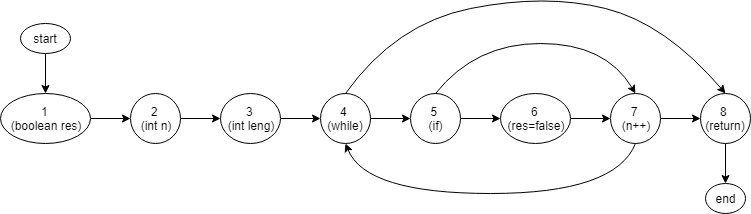
\includegraphics[width=0.67\paperwidth]{foto/cfg.png}}
\caption{CGF taken from a sample binary provided as input to IDA Disassembler \cite{ida}}
\label{fig:cfg}
\end{figure}

\newpage
This is usually done by creating a "Control Flow Graph" (CFG) of the program, i.e. a representation in graph notation of all paths available during a single execution flow: each node in the graph represents a "basic block", i.e. a sequence of instructions or statements with no jumps, and the edges between nodes represent jumps, loops and branch construct (if-else) in the program's execution (see figure \ref{fig:cfg}). By analyzing a single execution flow and measuring the number of nodes and edges traversed, the number of functions triggered, and which branches were activated during conditional statements, the fuzzer keeps track of all paths that have yet to be explored, providing useful information when generating new testcases. 

Therefore, we define \textit{interesting input} as any testcase that increases the code coverage achieved in a fuzzing session, and it is used as a reference when generating new testcases to hopefully get even more coverage.


\subsection{What is a fuzzer}  \label{fuzzers}
A \textit{fuzzer} is the tool performing fuzz testing, taking as inputs the program being tested and a set of testcases that will be used during the fuzzing session. It is responsible for executing the program against all the provided inputs in an automated manner, analyze each execution for potential unwanted behavior and produce new and useful testcases for future fuzzing session that will attempt to trigger new execution flows and even more bugs.
\begin{figure}[h]
\centering
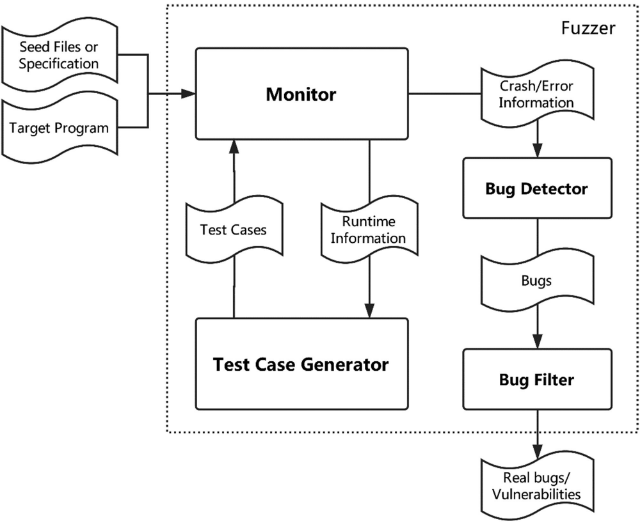
\includegraphics[scale=0.46]{foto/fuzzing_workflow.png}
\caption{General fuzzing workflow \cite{fuzzing_survey}}
\label{fig:fuzzing_workflow}
\end{figure}

In general, a fuzzer is composed by the following key elements \cite{afl_docs} \cite{fuzzing_survey}.

\textbf{Target program.}\ \ \ Refers to the program that is being tested: it could be either binary or source code, although source code of real-world software is usually not accessible.

\textbf{Program's Specification}\ \ \ Some fuzzers can receive as input the program's specification, i.e. a formal description of the target program and its behavior using as the available documentation and source code, and translate its functionalities and expected behavior using a specific grammar that the fuzzer understands. However, this information is rarely available and often too difficult to infer without the appropriate data.

\textbf{Observer (or Monitor).}\ \ \ Provides runtime information observed during the execution of the target to the fuzzer, leveraging techniques such as code instrumentation, taint analysis, code coverage and many more. Such information may be relatively simple, like the total running time for a test and its output, to more advanced ones, like the maximum depth of the stack. They are usually not preserved across many execution, unless an "interesting input" is encountered, in which case they are relayed to the \textit{Test case generator}  to be used as reference during the generation of new testcases. 

\textbf{Executor.}\ \ \ Responsible for defining how the program will be executed and the arguments passed on each run. The input for a single test is provided either by writing it in some specific memory location or passed as argument to a so called "harness function", although each fuzzer has its own implementation of this element. Given this, we briefly mention few standard functionalities that compose this element. The \textit{InProcessExecutor} runs the "harness function" and provides crash detection. The \textit{ForkServerExecutor} is responsible for spawning different child processes to fuzz. The \textit{TimeoutExecutor} wraps and installs a timeout for another running executor.

\textbf{Test case generator.}\ \ \ Performs generation of new testcases to increase code coverage using runtime information received from the observer and \textit{interesting inputs} as reference. This can be done using either \textit{mutation} or \textit{generation}, depending on the type of fuzzer chosen (discussed later), although it's important to note that there is no one-size-fits-all solution.

\textbf{Feedback.}\ \ \ Chain of components that classify the result of a single execution and determine if the initial input is "interesting" or not analyzing the information received from the observers and the updated coverage map. Some examples shown in figure \ref{fig:fuzzing_workflow} are the \textit{Bug Detector}, that collects and analyze debug information during crashes and errors, and the \textit{Bug Filter}, which classifies the errors collected.
Each component of this chain usually has its own objective (crashes, timeouts, new execution flows discovered, assertions), and combining them in boolean expression allows the developer to collect more fine-grained results and maximize a desired target function.

\textbf{Testcase.}\ \ \ Data taken from an external source and provided as input to the tested program to observe its behavior, usually in the form of bytes arrays. Each testcase is defined by a set of metadata like ID, description and expected results. The first fuzzing session takes a set of inputs that is defined and provided by the developer itself, while future fuzzing session will also rely on previously discovered "interesting inputs". 

\textbf{Corpus.}\ \ \ Location where testcases are stored, usually disk or memory. An example of input corpus may be composed by several testcases with the same properties, like crashing the program under a specific situation. An example of output corpus may be composed by all the testcases that are considered "interesting" or a collection of all inputs that triggered a bug in the program.








\newpage
Fuzzers can be then categorized using the 3 following characteristics.

\textbf{Input generation.}\ \ \  During each fuzzing session, one of the most important operations performed by the fuzzer is the generation of new testcases, with the objective of diversifying and increasing the effectiveness of the corpora that will be used on future fuzzing sessions: more specifically, an effective fuzzer should be capable of generating inputs "valid enough" so that they are not rejected from the program's parsers, but also "invalid enough" to potentially trigger corner cases. Given this, we  distinguish between \textit{mutation-based} and \textit{generation-based} fuzzers. The \textit{mutation-based fuzzers} require an initial seed of inputs as reference, and the generation of new inputs is performed by applying "mutators" on the provided seeds: these operations range from flipping/adding/removing bits (or bytes), performing mathematical operations and sometimes even completely randomizing its content. Finally, these mutations are usually mixed forming sequences to increase randomness. The \textit{generation-based fuzzers}, instead, rely on a good source of randomness to generate new inputs from scratch, and for this reason they do not depend on the existence of a good initial corpus nor on its quality, although they require more starting time before the tests become effective.

\textbf{Input's structure awareness.}\ \ \ Another information useful to the fuzzer, although not always available, is the "input model", i.e. the correct structure that a file must have when testing programs that follow rigorous standards. However, not all of them provide this feature, and for this reason we define \textit{smart} and \textit{dumb} fuzzers.
A \textit{smart mutation fuzzer} might leverage this knowledge to switch between different types of inputs, while a \textit{dumb mutation fuzzer} can only rely on the structure of the "interesting inputs" and apply limited random mutations, usually resulting in a much lower proportion of valid inputs being generated.
A \textit{smart generation fuzzer} uses this information to avoid wasting resources on generating inputs that are too random to be accepted, as the \textit{dumb generation fuzzer} attempts to generate new inputs without any reference, oftentimes putting more stress on the program's parser rather than the program itself due to the overwhelmingly high number of invalid inputs generated in the first phases.

\textbf{Program's structure awareness.}\ \ \  Fuzzers may be accompanied by program analysis' techniques to increase the efficiency and effectiveness of the tests. A \textit{black-box fuzzer} is completely unaware of the program's structure, therefore assumes the program as a simple machine that takes a random input and generates an according output: this approach is relatively fast, can be easily parallelized and has good scalability, however it will most likely find only bugs that do not require particular conditions to be met to be triggered, also called "surface bugs". A \textit{white-box fuzzer} employs program analysis' techniques to systematically explore and reach critical program locations through meticulously crafted inputs, allowing you to discover bugs that could be potentially hidden deep in the program: while this approach is arguably the most effective one, it implies that bugs related to unknown aspects of the program can be easily missed, and the time used to analyze the program as well as generating such specialized input exponentially increases with the program's complexity.
A \textit{gray-box fuzzer} attempts to find a balance between efficiency and effectiveness by integrating the best aspects of both approaches: using a minimal amount of knowledge over the program's structure to achieve a sufficient degree of code coverage such that the results obtained are satisfactory.



\newpage
A \textit{fuzzing session} defines the process of testing a program using a fuzzing tool.
Assuming the program has been properly compiled using the chosen fuzzer, the first step is to simply start the fuzzing session and let the fuzzer execute the program on many different testcases. After some time, when either the initial corpus has been exhausted (mutation-based) or the fuzzer learned what is an acceptable inputs (generation-based), it starts applying random operations to generate new testcases. 

During each execution, code coverage and unexpected behaviors are tracked, so that all testcases that increases any of these statistics will be regarded as "interesting inputs" and saved in a separate queue. In this context, the fuzzer has to be sensible enough to distinguish between crashing and non-crashing inputs without having full knowledge over the program tested, and therefore \textit{sanitizers} are used to "instrument" the source code and inject assertions that make the program crash when a particular kind of failure is detected. Section \ref{sanitizers} explains this concept more thoroughly.

At the end of each fuzzing session, the user is presented with three results: a collection of statistics regarding the coverage achieved and bugs found, a list of inputs that caused crashes along with some metadata (testcase ID, bug type, memory state, etc...), and a set of "interesting inputs" that can be used in future fuzzing sessions to provide the fuzzer with even more information about the structure of a good input that explored the deepest parts of the program. 
The statistics provided may be useful to understand how effective this particular fuzzing session was with respect to the previous ones, if the initial corpus needs to be refined and whether the changes applied to the code have been fruitful or not.
The new set of "interesting inputs" is then added to the existing initial corpus, which in turn is \textit{pruned}: this process removes any duplicates and inputs that trigger the same execution flow or bugs, which is crucial to ensure that the size of the corpus does not explode over time.
Finally, the developer has to analyze all the inputs that caused a bug and perform \textit{bug triage}: execute each input individually to observe its output, determine which kind of error occurred and why, fix the bug entirely (if possible) or at least patch the problem, and ensure that the bug does not occur in future fuzzing sessions by including the triggering input(s) in the set used for the tests.

All these steps are repeated across many different fuzzing sessions, sometimes even changing the scope of the tests to increase code coverage or stressing the program with many buggy inputs, each time making the program more secure against vulnerabilities and more robust to extraneous inputs. 

In conclusion, many modern fuzzers originate from a solution that represented a breakthrough in fuzzing research called \textit{American Fuzzy Lop} (also known as \textit{AFL} \cite{afl}), a "dumb mutation-based fuzzer" that achieved many results over the years: in September 2014 it discovered "Shellshock" \cite{shellshock} (also known as "Bashdoor"), a family of security bugs affecting the Unix Bash shell that allowed malicious users to execute arbitrary commands without confirmation, while in April 2015 it discovered the famous "Heartbleed" \cite{heartbleed} bug in OpenSSL, which allowed malicious users to decipher the otherwise encrypted communications used by the TLS protocol.
Since 2017, when the development of this tool was stopped, there have been many variants and improvements of this tool, and some honorable mentions are WinAFL \cite{winafl}, VUzzer \cite{vuzzer}, FairFuzz \cite{fairfuzz}, Fuzzolic \cite{fuzzolic} and QSYM \cite{qsym}. This thesis focused on AFL++ \cite{AFL++}, a direct fork of AFL with new and better mutation and coverage algorithms, which is considered to be the current state-of-the-art fuzzer.







\newpage
\section{Sanitizers} \label{sanitizers}
A \textit{code sanitizer} is a tool used to detect bugs in a program during both compilation and runtime, with different sanitizers specializing in detecting different kinds of bugs: misuse of addresses, stack- and heap-overflows, use of uninitialized memory and leaks as well as undefined behavior.

They are added to a program through "instrumentation", which refers to modifying either the source code or the binary code to introduce some additional functionalities and references that can be used by other tools to perform code analysis, logging or profiling. Although code sanitizers should be a standard practice in the development cycle of a program, unfortunately this is not the case as introducing these tools not only requires extensive tests to check for potential errors, but also because they do not always interact very well with shared libraries or other external dependencies. It is also extremely important to mention that these bug detection tools are not meant to be linked against production executables, as their runtime was not developed with security-sensitive constraints and may compromise the security of the released product \cite{asan_docs}\cite{msan_docs}\cite{ubsan_docs}.

A \textit{compile sanitizer} is a tool that performs instrumentation at compile-time, meaning that it introduces functions and libraries that will be then added and compiled together with the original source code, effectively altering its default behavior. Their advantages are twofold: they are able to achieve full coverage and provide warnings and errors during the compilation process, since the analysis is performed directly on the source code and includes all possible paths, and they are also able to detect errors during the execution of the program, although obviously limited by the single execution flow analyzed. However, these sanitizers introduce a non-trivial overhead both in terms of increased compile time, execution time and memory usage, which may cause problems when it comes to managing computing resources.

A \textit{binary sanitizer} is a dynamic binary instrumentation (DBI) framework that performs "Just-in-Time" (JIT) compilation to introduce additional instructions and analysis callback during the execution of a program, effectively without modifying the original code, and they often rely on dynamic binary analysis (DBA) tools to analyze programs at run-time at the level of the machine code. Also these sanitizers are dependent on the input given and the resulting execution flow analyzed, therefore they are not capable of achieving full code coverage. Moreover, this analysis requires attaching another external process to instrument the original one, which usually causes massive slowdowns and sometimes might even break the original's code functionality.  

This work focused on using several compile sanitizers developed by Google \cite{san_repo} as part of its tool suit provided to open-source developers, along with a popular binary sanitizer \cite{valgrind_web} to perform a cross-check on the results produced by the compile sanitizers, as these tools have been proven to be particularly effective when combined with fuzzing due to their ability to trigger bugs.




\newpage
\subsection{ASan and LSan}
The \textit{Address Sanitizer} \cite{serebryany2012addresssanitizer} is a memory error detection tool for C/C++ that helps developers to find and fix any out-of-bounds accesses to heap, stack and global objects, use-after-free bugs and provides protection against stack-based and heap-based overflow, making it one of the most popular and effective sanitizers.

When allocating bytes for a buffer and performing an access beyond such boundaries, a program will usually crash with an "out-of-bounds exception", but it could also happen that it is valid to access information in the unallocated address, in which case the program will crash unexpectedly and make it difficult for the developer to understand the problem. Moreover, if such addresses are not properly freed, they could leave a so called "dangling pointer", and thinking that this memory location still holds valid data (maybe even confidential one) implies serious security issues.
If an attacker discovers a program with such vulnerabilities, he could use them to crash the application, corrupt or retrieve sensitive data, or even perform a "remote code execution" attack by inserting some malicious code via this buffer overrun and causing the program to jump and execute that particular memory location, creating an attack vector where anything is possible. 

To prevent this, the sanitizer uses a shadow memory to map the memory regions allocated by the application and record whether each byte of such areas can be safely accessed by load/store operations. Each memory region is assigned a shadow counterpart, containing metadata about its size and the offset range that can be used to safely access it, while any attempt to read/write beyond such boundaries will trigger a sanitizer error, as shown by the figure below:

\begin{figure}[h]
\centering
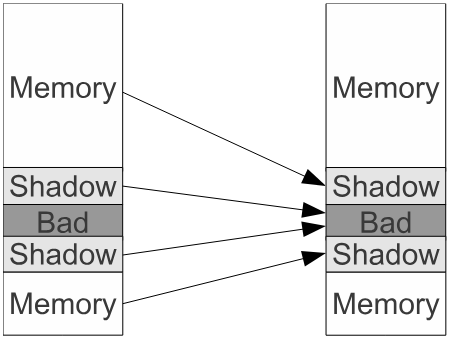
\includegraphics[scale=0.6]{foto/shadow_memory.png}
\caption{Memory mapping of ASan \cite{serebryany2012addresssanitizer}}
\label{fig:asan_shadow}
\end{figure}

Detection of out-of-bounds accesses to globals and stack objects is done in a similar way, i.e. by creating poisoned memory regions around such objects: \textit{global variables} are poisoned at compile-time and their addresses computed during the application startup, while \textit{stack objects} are poisoned and recorded at run-time.

The management of the shadow memory is done by ASan run-time library, containing specialized implementation of the \verb|malloc| and \verb|free| functions, which allocate extra memory for shadow and poisoned memory zones as well as keeping a FIFO stack of allocated and freed memory regions to detect use-after-free, double-free and invalid-free bugs.

This sanitizer is also provided with another component called \textit{Leak Sanitizer} (or \textit{LSan}), a memory leak detector enabled by default that returns which portions of the program are leaking memory as well as the size leaked, thanks to comprehensive and exhaustive stack traces. A memory leak is a condition where a program fails to release memory that is no longer needed due to developers' negligence or software error, effectively reducing the amount of memory available by the machine, and this will inevitably lead to performance degradation (trashing). Although this component may seem very helpful, it usually generate huge logs especially when having complex programs that heavily rely on external libraries, which oftentimes do not perform clean releases of the objects used.

Finally, ASan adds a slight overhead, increasing execution times by an average 170\% and memory usage by 3.4x \cite{serebryany2012addresssanitizer}.





\subsection{MSan}
The \textit{Memory Sanitizer} \cite{stepanov2015memorysanitizer} is a memory reads detector for C/C++ that helps developers to find and fix use-of-uninitialized-memory (UUM) bugs, which are considered to be quite tricky as they do not necessarily occur in every execution and could be triggered by any operation performed by the program. This is because the C/C++ languages are defined "memory-unsafe" due to the fact that the management of the memory is left to the developer, who is responsible for correctly allocating, using and freeing any memory region that is accessed by the program: in fact, unless specified, any new allocation operation performed by these languages creates uninitialized stack and heap objects. Such vulnerabilities may not only be exploited to alter the execution flow and inject malicious code, but also to leak information about a program's internal stake, such as the content of the stack or heap.

A UUM bugs usually originates from any operation that loads a value from an uninitialized memory region, resulting in an \textit{undefined value} being returned, and operations like conditional branch, syscall and pointer dereference are most likely to trigger them. This sanitizer works by using a shadow memory to map each bit of application memory and encode its state (0 initialized, 1 otherwise): all newly allocated memory is poisoned, i.e. the corresponding shadow memory is initialized to \verb|0xFF|, and "shadow propagation" operations are performed to safely copy an uninitialized variable to different memory regions as well as safely perform simple logic and arithmetic operations on them without occurring in errors.

\begin{figure}[h]
\centering
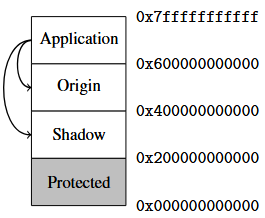
\includegraphics[scale=0.8]{foto/shadow_memory_2.png}
\caption{Memory mapping of MSan \cite{stepanov2015memorysanitizer}}
\label{fig:msan_shadow}
\end{figure}

Given that UUM bugs are notoriously hard to reproduce and debug, MSan provides the "origin-tracking-mode" to obtain more comprehensive and descriptive stack-traces. If necessary, there is also the "advanced-origin-tracking-mode", which records the entire stack and all operations that happen between the allocation and load of uninitialized variables, but its usability is still discussed due to the huge amounts of memory it requires.

The management of the shadow memory is done by MSan run-time library, that maps the "shadow" and (optional) "origin" areas and marks as uninitialized any new allocated regions as well as the deallocated ones. To update the shadow region, a large subset of the standard \verb|libc| functions are intercepted.

Fixing these bugs generally requires little to none effort, but many developers avoid this sanitizer due to the huge slowdown that it introduces. In fact, MSan increases execution times by an average 300\% and memory usage by 2x on short programs, values that rapidly worsen with complex programs \cite{stepanov2015memorysanitizer}.





\subsection{UBSan}
The \textit{Undefined Behavior Sanitizer} \cite{ubsan_docs} is a fast undefined-behavior detector for C/C++, that helps developers to find and fix undefined-behavior (UB) bugs. The C language specification allows developers to perform many complex and (sometimes) unreasonable operations on the assumption that they know what they are doing, and this leads to the compiler making arbitrary decisions when the code does not conform to some expected values: for example, an array indexed with an out-of-bound value will not always crash the program if said memory location contains valid content that belongs to the program, while performing a conversion between two data types of different sizes will result in unpredictable loss of data due to rounding operations. This means that different compilers will handle such situations differently and produce unexpected results each time they are executed, all without taking into account that the hardware used and the level of optimization chosen will also affect these results.

Common operations that may lead to undefined behaviors are: array subscription out of bounds, overflows/underflows of numerical types due to mathematical or logical operations, shifts of numerical values, dereferenced, misaligned or null pointers and invalid conversions between data types. Although this list is not exhaustive of all possible scenarios, it is apparent that most of the problems mentioned could be fixed with negligible effort and avoided altogether by applying appropriate coding standards.  

This sanitizer works similarly and sometimes overlaps with ASan, putting protected regions around buffers and inserting correctness-checking functions after all mathematical, logical and implicit/explicit cast operations. By default, due to its simplistic nature, the tool does not print stack-traces and uses a minimal run-time library, although the "print-stacktrace-mode" option can be enabled to obtain more comprehensive results.

To conclude, UBSan adds a trivial overhead, increasing execution times by an average 120\% and memory usage by 2x \cite{ubsan_docs}.



\subsection{Valgrind}
Valgrind is a Dynamic Binary Instrumentation (DBI) framework for building dynamic analysis tools, i.e. tools that perform code analysis at runtime, and is capable of achieving full coverage of user-mode code. It is distributed with seven production-quality tools that perform code profiling, memory analysis and threading bugs, with similar functionality to ASan and MSan \cite{valgrind_web}.  

The tool relies on dynamic binary recompilation to load the client program into the \textit{Valgrind Core} and (re)compile the client's machine code in small blocks using a "Just-In-Time" (JIT) approach, producing a so-called "Intermediate Representation" (IR) which is then instrumented with analysis code. This translated code is then stored in a code cache, so that it can be rerun when necessary avoiding this overhead. It is also capable of monitoring the CPU registers during the program execution by taking control of the real CPU and (conceptually) running the client program on a simulated one, and the concept of "shadow memory" is used to analyze and protect both memory and CPU registers \cite{Valgrind_1} \cite{Valgrind_2}.

This work relied on Valgrind's memory-analysis tool called \textit{Memcheck} \cite{memcheck_docs}\cite{memcheck_paper}, a memory-error detector for C/C++ program when performing accesses to heap and stack elements, use of uninitialized and undefined values, incorrect allocation and freeing of heap memory, misuse of allocation functions and finally tracking memory leaks. Since most of its functions overlaps with MSan, it was used as a replacement for detecting UUM bugs when analyzing projects that relied heavily on external libraries: this is because, of the compile sanitizers mentioned above, MSan is the only one that requires all libraries linked to the executable to be rebuilt with this sanitizer in order to get meaningful results. However, this process proved to be too cumbersome and beyond the scope of this work, also because most projects used statically linked libraries rather than compiling them from scratch.

While Valgrind is a very popular and widely used tool, it also suffers from a major limitation due to its design choice, which is that it is a single-threaded program: this means that its execution cannot be parallelized and the entire program and its analysis run on a single CPU core and kernel thread. In fact, Valgrind applies an average slowdown of 4x by default, value that can range from 10x up to 100x for CPU-bound programs when other analysis tools are introduced \cite{Valgrind_1}: for example, the Memcheck tool introduces a slowdown between 20x-30x for most programs \cite{memcheck_docs}.





\newpage
\section{Open-Source Software}
The \textbf{Open-Source Software (OSS)} is a computer software developed in a collaborative and public manner, released under a particular license that allows other users to freely use, study, modify and distribute the software and its source code for any purpose: this allows many users to actively participate in the development of a software by proposing changes and new improvements.
To be eligible as an open-source software, the license's distribution terms must comply with several criteria \cite{osd}: the main concept is to let anyone easily download your program and access its the source code, allowing them also to modify and redistribute the project without additional fees as long as the original code is appropriately credited. 

Given all this, one could argue that making all this information publicly available poses a real threat to security: history has shown us many times that, given enough time and resources, releasing the source code of a program will result in malicious users discovering bugs and vulnerabilities that could have potentially catastrophic consequences. 

For this reason, we mention some key aspects that should be considered when approaching open-source software.

\textbf{Development.}\ \ \ Open-source software is usually released under two development branches: a "stable" version, composed by all the functionalities that have been thoroughly tested and work as intended, and a "build" version, that is slightly buggier as it includes proposed changes and new features that have yet to be refined. Releasing the "build" version early not only allows the developers to showcase their work and attract even people, but also provides them with feedback from real users that are willing to run untested versions of their software.

\textbf{User interaction.}\ \ \ Providing full access to the source code means that other users might want to contribute in the program's development and help the developers in improving and refining the product: considering that each user may have different knowledge and programming skills as well as different testing environments, this allows them to test and benchmark the product on a wide range of systems, further increasing the probabilities of finding new and unknown bugs that may be specific to a single OS or architecture.

\textbf{Bug reporting.}\ \ \ Although any user has the rights to mention a bug, error, or mistake in the program or the documentation, it is still up to the developers to ensure the truthfulness of what has been reported and how to tackle it. For example, bugs that are not security-relevant or that may be related to QoL aspects are easily pushed back as secondary problems or simply ignored altogether. Sometimes, if the developer are kind enough to accept your request but do not have time and resources to solve it, they might ask for a proposed fix and cite the user themselves in the next patch notes as a way of thanking them.



\newpage
\section{Continuous Fuzzing}
In the past decade, fuzzing became one of the most popular dynamic automated testing techniques, with both small and large companies employing it to discover bugs and vulnerabilities in their products. However, a fuzzing session needs to run for at least 24 hours \cite{evaluating_fuzz} to produce meaningful results, and time is a resource that most organizations cannot afford to lose. For this reason, they often employ short but continuous fuzzing campaigns together with a software development paradigm called \textit{CI/CD pipeline} (\textit{Continuous Integration} and \textit{Continuous Delivery}): CI refers to the practice of frequently integrating and testing changes to the source code to ensure that the product is always in a well-functioning state. CD is a delivery strategy in which software is developed in short tasks and released with incremental updates, helping developers to reduce costs by making development simple and repeatable, but also avoiding unnecessary risks from applying too many changes at once. 

In general, a continuous fuzzing framework refers to an automated framework that integrates any changes committed to the code, builds and tests debug versions of the program with one (or more) configuration of fuzzers and sanitizers, and finally deploys a new version of the product to end users. To further increase early defect discovery, many of these frameworks rely on a technique called \textit{ensemble fuzzing}, with a workflow similar to the one shown below:

\begin{figure}[h]
\makebox[\textwidth][c]{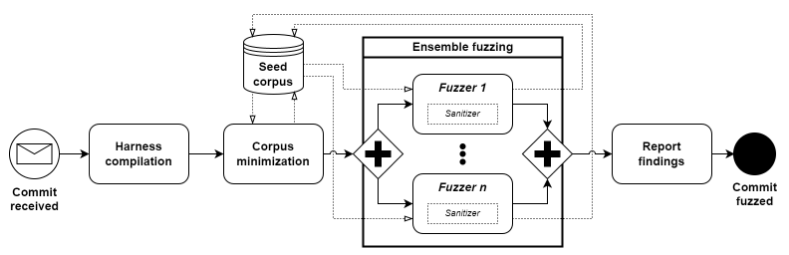
\includegraphics[width=0.75\paperwidth]{foto/ensemble_fuzzing.png}}
\caption{Generic design of ensemble fuzzing in a CI/CD pipeline \cite{continuous_fuzzing}}
\label{fig:continuous_fuzzing}
\end{figure}

Instead of focusing on testing a program with a single fuzzer (along with sanitizers) for several hours, this approach focuses on testing the same program in short sessions with different combinations of fuzzers and sanitizers, mixing and matching mutation-based and generation-based fuzzing tools. Each fuzzer runs asynchronously and separately from the others, collecting interesting inputs and applying its own operations to generate new inputs. Then, all results are collected and synchronized into a single queue for analysis and use in subsequent fuzzing sessions: this approach maximizes both the diversity of inputs used, as each fuzzer will be using testcases produced by other fuzzers, and the diversity of results, as each fuzzer will test code differently potentially leading to the discovery of new bugs. Of course, in order to use this technique, developers must compile and prepare the binaries accordingly.

\newpage
We briefly mention few popular continuous fuzzing infrastructures. Microsoft announced in 2020 the \textit{Project OneFuzz Framework} \cite{onefuzz}, an extensible and open-source self-hosted fuzz testing framework with the goal of enabling developers to easily and continuously fuzz programs prior to their release, while scaling fuzzing workloads in the cloud thanks to Azure. It enabled developers to build and compose a continuous fuzzing workflow using several fuzzing tools, automatic bug triage and results deduplication and a multi-platform design. Unfortunately, its development was stopped as of September 2023 \cite{onefuzz_repo}. GitLab provides continuous coverage-guided fuzz testing as part of its CI/CD services \cite{gitlab_fuzz}, supporting many different languages and fuzzing engines. Google provides \textit{ClusterFuzzLite} \cite{google_lite_repo}, a continuous fuzzing solution as part of CI workflows to fuzz pull requests and catch bugs before they are committed \cite{google_lite}, and \textit{OSS-Fuzz} \cite{ossfuzz_paper}, a continuous fuzzing service for open-source software.

Google was also one of the first major companies that connected automated testing, continuous fuzzing frameworks and open-source software together. The \textit{Google Open Source Project} \cite{google_oss} is a campaign started in 2004, one of the oldest open-source campaigns in the industry: it was initially meant to share Google-developed software under open licenses, with the intention of bringing free technology and information sharing to the public, but it quickly became a program dedicated to improving open-source ecosystems as a whole. Thanks to this campaign, many projects became popular and gained worldwide recognition such as Android OS, TensorFlow, the Go programming language, and many more.

This thesis will focus on two campaigns maintained by Google called \textit{OSS-Fuzz} \cite{ossfuzz_docs} and \textit{FuzzBench} \cite{{fuzzbench_docs}}: the first is a free platform that allows open source developers to fuzz their programs autonomously by integrating with existing CI/CD pipelines and relying on the computing resources provided by the Google Cloud Service, while the second allows fuzzer developers to test and improve their tools against real-world benchmarks thanks to automated testing and reporting. The objective was to test a selected group of the projects that have been implemented in these repositories using alternative approaches, trying to discover bugs that will be then securely reported and disclosed to their developers in hope to have them fixed.

\subsection{ClusterFuzz}
Before introducing the frameworks mentioned above, it is also important to define the underlying infrastructure. The \textit{ClusterFuzz Project} is a scalable fuzzing infrastructure with the objective of discovering security and stability issues in software through continuous coverage-guided fuzzing, it is also the main platform used by Google to test its own products and the fuzzing back-end for \textit{OSS-Fuzz}. As of May 2023, it discovered over 25.000 bugs in Google proprietary software (e.g. Chrome) and 36.000 bugs with OSS-Fuzz \cite{clusterfuzz_docs}.

It is based on a highly scalable distributed system of VMs that performs fully automated fuzzing, bug triage, filing and closure of bug reports as well as providing performance statistics, and all operations are performed by two main components.
The \textit{App Engine} provides a web interface to the information collected during each fuzzing session, allowing the developers to easily access crashes, results and other information. This is also where tests can be scheduled, which is done via \verb|cron| jobs.
The \textit{Fuzzing Bots Pool} is a cluster of VMs responsible for running the scheduled fuzzing sessions, and they perform the following operations:
\begin{itemize}
    \item \textbf{fuzz:} runs a fuzzing session
    \item \textbf{progression:} checks if a testcase still reproduces or if has been fixed
    \item \textbf{regression:} calculates the commits range in which a crash was introduced
    \item \textbf{minimize:} eliminates duplicate testcases from the input seeds
    \item \textbf{pruning:} minimize a corpus to the smallest size based on coverage information
    \item \textbf{analyze:} runs a manually uploaded testcase against a specific job to see if it crashes
\end{itemize}

\begin{figure}[h]
\makebox[\textwidth][c]{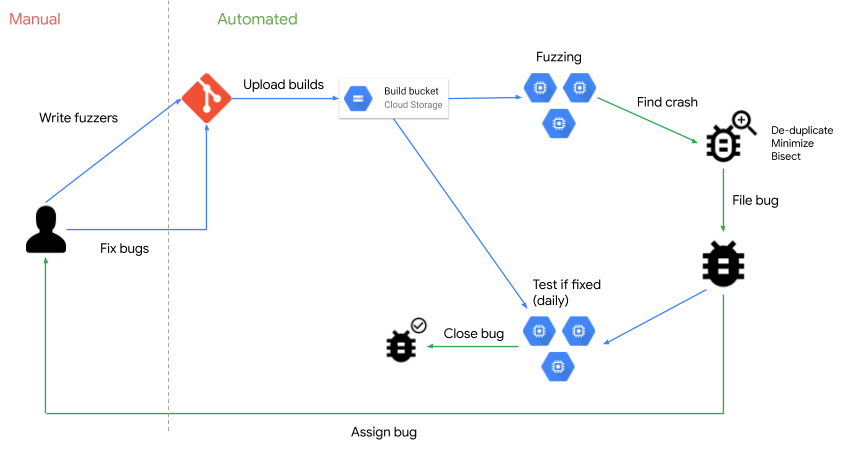
\includegraphics[width=0.64\paperwidth]{foto/clusterfuzz_architecture.png}}
\caption{ClusterFuzz main architecture visualized \cite{clusterfuzz_docs}}
\label{fig:clusterfuzz_architecture}
\end{figure}

Each VM performs these operations inside Docker instances created and uploaded by the developers, which are configured with all the tools and files necessary to correctly build and launch the fuzzing targets. Since some of these tasks are critical and should be treated as atomic operations, bots can be \textit{preemptible} or \textit{non-preemptible}: the former refers to a machine that can only run the "fuzz" task as it can be shut down at any moment, while the latter refers to a machine that is not expected to suddenly stop or crash and is therefore capable of performing all tasks.



\subsection{OSS-Fuzz}
The \textit{OSS-Fuzz Project} \cite{ossfuzz_paper} was founded in 2016 after the famous "Heartbleed" vulnerability was discovered in OpenSSl, one of the most popular open-source projects at the time for encrypting web traffic, as a response to provide developers with free fuzzing and private alerts services for their open-source projects. As of August 2023, it has helped identify and fix more than 10,000 vulnerabilities and 36,000 bugs in over 1000 projects \cite{ossfuzz_docs}.


While it was initially intended for languages that are not memory-safe (C/C++), it was later extended to provide support also for other popular languages such as Python, Go, Java and Rust. Projects can be tested using several coverage-guided mutation-based fuzzing engines (such as LibFuzzer, AFL++ and Honggfuzz) in combination with Google Sanitizers (ASan, MSan and UBSan), while \textit{ClusterFuzz} acts as the back-end and provides bug reporting functionalities.

\begin{figure}[h]
\makebox[\textwidth][c]{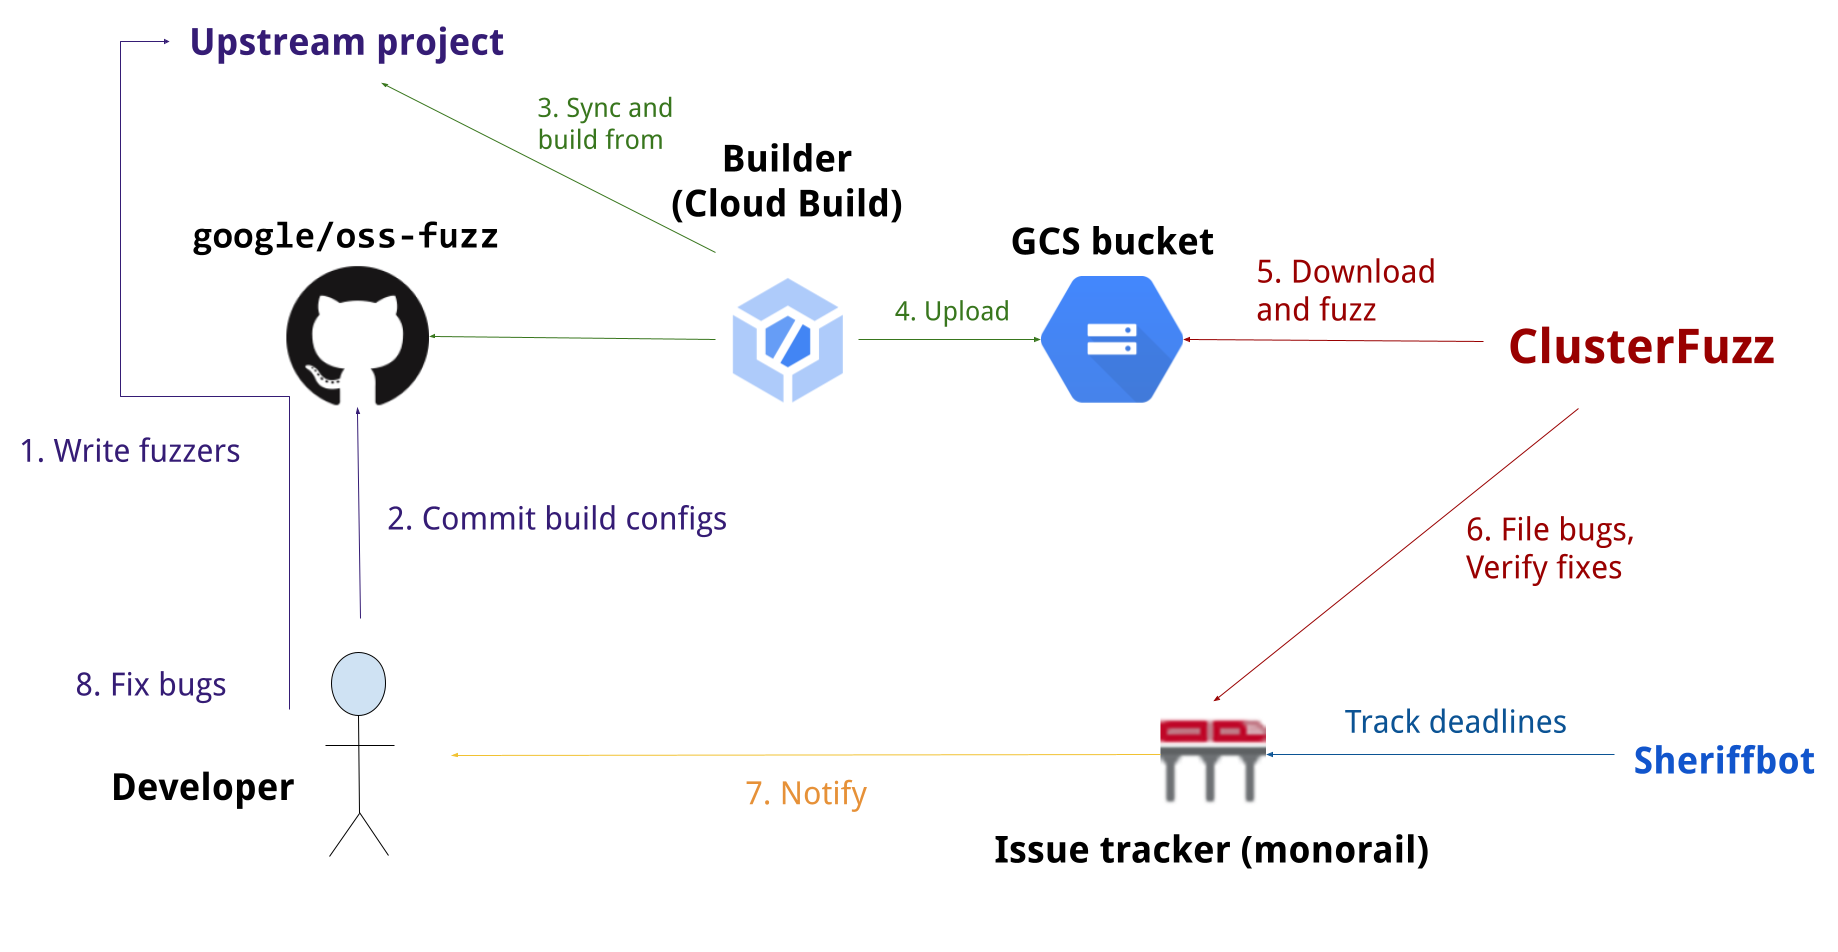
\includegraphics[width=0.65\paperwidth]{foto/oss-fuzz_architecture.png}}
\caption{OSS-Fuzz main architecture visualized \cite{ossfuzz_docs}}
\label{fig:ossfuzz_architecture}
\end{figure}

The workflow is as follows. First, the maintainers of an open-source project create one or more "fuzz targets" that are integrated into the project's build and test system \cite{libfuzzer_docs}, where a "fuzz target" defines a function that takes an input (in this thesis, an array of bytes) and performs some operations on said to test a specific API or program's functionality. Developers are also expected to provide up-to-date corpus seeds, that will be used by the chosen fuzzers for cross-mutations and improve the fuzz target’s coverage. All these resources, along with instructions on how to build and fuzz the targets, are uploaded to a Google Cloud Service Bucket, a file-hosting service acting as a middle point between OSS-Fuzz and its fuzzing back-end ClusterFuzz.

Then, a project's fuzzing session lasts (at most) 6 hours, evenly distributed across all fuzz targets with a minimum of 10 minutes per fuzz target, and \textit{ensemble fuzzing} is used when binaries are configured for multiple fuzzing engines (see figure \ref{fig:continuous_fuzzing}). Both the corpora used as input to the tests and the corpora produced as results of a successful fuzzing session (both also called \textit{queues}) are publicly available and stored in the project's Google Cloud for research purposes and \textit{regression testing}, i.e. testing a program against old inputs to ensure that previously tested functionality still works as intended and that fixed bugs do not reappear.

Finally, any bug discovered is reported to the OSS-Fuzz issue tracker \cite{ossfuzz_bugtracker}, which uses the metadata sent by ClusterFuzz to create its report. Developers have 3 ways of dealing with this situation: they can commit new changes to fix the bug (verified by ClusterFuzz before closing an issue), assign the tag "WontFix" to the bug and notify that it will not be solved, or simply ignore it altogether. 



\newpage
To be accepted by OSS-Fuzz, a project must be relevant and/or critical to the global IT infrastructure and it must have a significant user base: to check if your project is eligible, Google provides a mathematical formula to calculate its "Open-Source Project Criticality Score" \cite{score} in a range between 0 \textit{(least critical)} and 1 \textit{(most critical)}, where $\alpha_i$ refers to the "weight" of an indicator and $T_i$ to its maximum allowed value:

\begin{equation}
    CriticalityScore = \frac{1}{\sum \alpha_i}\  \sum_i \alpha_i \ \frac{\log(1+S_i)}{\log(1+\max(S_i,T_i))}
\end{equation}
\ \\
The parameters evaluated are the followings:
\begin{itemize}
    \item \textbf{created-since} ($\alpha_i = 1$, $T_i = 120$): months since the project was created, older projects have a higher chance of being widely used or dependent on
    \item \textbf{updated-since} ($\alpha_i = -1$, $T_i = 120$): months since the project's last update, unmaintained projects with no recent commits have a higher chance of being less relied upon
    \item \textbf{contributor-count} ($\alpha_i = 2$, $T_i = 5000$): number of commits made by project contributors, involvement of different contributors indicates a project importance
    \item \textbf{org-count} ($\alpha_i = 1$, $T_i = 10$): number of distinct organizations contributing to the project, indicates cross-organization dependency
    \item \textbf{commit-frequency} ($\alpha_i = 1$, $T_i = 1000$): average number of commits per week over the last year, code that is constantly changing may be more susceptible to vulnerabilities
    \item \textbf{recent-releases-count} ($\alpha_i = 0.5$, $T_i = 26$): number of releases in the last year, frequent releases indicate user dependency
    \item \textbf{closed-issues-count} ($\alpha_i = 0.5$, $T_i = 5000$): number of issues closed in the last 90 days, indicates contributor involvement and focus on resolving user issues
    \item \textbf{updated-issues-count} ($\alpha_i = 0.5$, $T_i = 5000$): number of issues updated in the last 90 days, indicates high contributor involvement
    \item \textbf{comment-frequency} ($\alpha_i = 1$, $T_i = 15$): average number of comments per issue in the last 90 days, indicates user activity and dependence
    \item \textbf{dependents-count} ($\alpha_i = 2$, $T_i = 500000$): number of project mentions in the commit messages, indicates repository use
\end{itemize}
\ \\
Only projects scoring a value $\geq 0.7$ may be eligible to be integrated in the OSS-Fuzz campaign.


\newpage
Assuming your project satisfies the score requirements, developers issue a "pull request" on the OSS-Fuzz repository providing the following 3 files, which are periodically checked and validated by a bot before accepting/rejecting them.

\paragraph{project.yaml} Configuration file that contains metadata regarding who owns the project, how to contact them when filing bug reports, and configuration parameters about the fuzzing sessions, needed by OSS-Fuzz to correctly provide its services.
Some of the most common information reported are:
\begin{itemize}
    \item \textbf{homepage:} URL to the project homepage
    \item \textbf{language:} programming language used to write the project (C, C++, Go, Rust, Python, JVM languages, Swift)
    \item \textbf{primary\_contacts:} list of email addresses that are automatically CC'd on crash reports and fuzzer statistics
    \item \textbf{main\_repo:} path to the source repository where the project is hosted
    \item \textbf{vendor\_ccs:} \textit{optional}, list of email addresses of vendors who want access to bug reports
    \item \textbf{sanitizers:} \textit{optional}, list of sanitizers available in the project (address, undefined, memory), if not specified "address" and "undefined" are used
    \item \textbf{architectures:} \textit{optional}, list of architectures that can build the project (supported only x86\_64 and i386)
    \item \textbf{fuzzing\_engines:} \textit{optional}, list of available fuzzing engines (libfuzzer, afl, honggfuzz and centipede), if not specified "libfuzzer" is used
    \item \textbf{builds\_per\_day:} \textit{optional}, number of times a project should be built per day, OSS-Fuzz allows up to 4 builds per day and builds once per day by default
\end{itemize}

\paragraph{Dockerfile} To avoid having developers create and maintain their own customized Docker containers and create an homogeneous and standard environment, OSS-Fuzz provides several "base images" based on Ubuntu 20.04 for each supported language, containing the most common compilers and toolchains needed to build the project and prepare the testing environment already installed. Each project builds its own testing environment starting from the most appropriate base image, runs a series of "apt-get" and "git clone" commands to download and install all the necessary packages and dependencies, and finally pulls all the resources and fuzz targets from the project repository.

\paragraph{build.sh} Script that runs inside the Docker container defined above and performs all the operations required to build the project and the fuzzing targets to be tested. To provide a more flexible and accessible build system, all base images are configured with several environment variables regarding directory locations, compilers and compilation flags, allowing developers to easily re-target scripts with little effort.


\newpage
To conclude, OSS-Fuzz follows a strict \textit{bug disclosure policy} \cite{bug_disclosure}.
When a bug is discovered (assuming it is not already known or a duplicate), an automatic email is generated and sent to all email addresses specified in the "project.yaml" file, and an issue is opened in the issue tracker. This email contains the report generated by ClusterFuzz, as well as an estimate of the priority and severity of the bug discovered. From this moment, the issue will be publicly visible in 90 days or after the fix is released (whichever comes earlier), meaning that anyone will have access to the causing input as well as any other debugging information related to what happened and how to reproduce the bug. Before the deadline expires, developers may request a 14-day grace period if the patch is scheduled to be released on a specific day within this extended period, in which case the public disclosure will be delayed. In all cases, Google reserves the right to move deadlines forward or backward depending on the circumstances and severity of the findings.




\subsection{FuzzBench}
The \textit{FuzzBench Project} \cite{fuzzbench_paper} is a free service that provides fuzzer developers with several real-world benchmarks tested at the Google scale, compares the results with other famous fuzzers (such as AFL and LibFuzzer), and allows them to evaluate their performance thanks to daily reports for further improvement \cite{fuzzbench_docs}.

\begin{figure}[h]
\makebox[\textwidth][c]{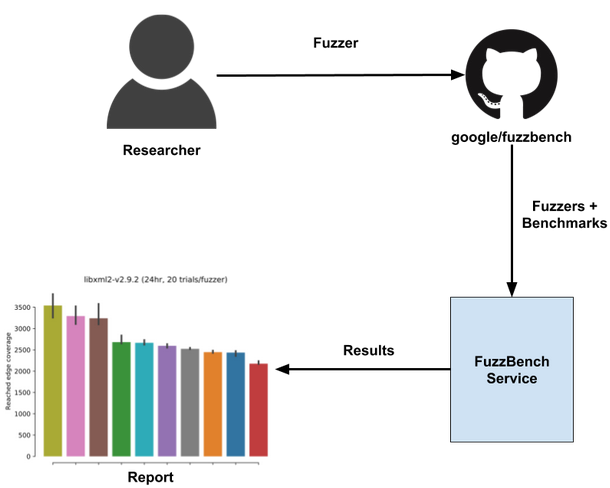
\includegraphics[width=0.7\paperwidth]{foto/fuzzbench_architecture.png}}
\caption{FuzzBench main architecture visualized \cite{fuzzbench_docs}}
\label{fig:fuzzbench_architecture}
\end{figure}

The infrastructure is structured as follows.
Initially, a fuzzer developer integrates its tool within FuzzBench using a Dockerfile, containing all the resources necessary to build targets using its fuzzer and also defining the environment where all benchmarks will be executed. Similarly to OSS-Fuzz, this process is done via "pull requests", which are automatically revisioned and accepted by bots.

Developers can then choose between two testing approaches: standard and OSS-Fuzz. In the former case, the benchmark is created by the developers themselves, which requires the definition of fuzz targets, build files, seed inputs and Docker images to correctly build, link the fuzzer to the targets and run the tests. In the latter case, the developers employ a fuzz target from a selection of OSS-Fuzz projects kept at a predefined checkout known to contain bugs \cite{benchmarks} with a predefined set of seeds inputs: this ensures that all tests are performed on the same version across many trials and with the same testing configuration, crucial to have a reference point when tracking performance over time, while also allowing them to test their product on a real-world scenario. A fuzzing session in FuzzBench spans over a duration of 24 hours, with each fuzzer running 20 trials on each individual benchmark.

Finally, a performance report will be created highlighting the strengths and weaknesses of the fuzzer on each benchmark, comparing individual and overall results with other integrated fuzzers both in terms of bugs found and coverage achieved.



\subsubsection{SBFT' 23}
FuzzBench already provides 21 open-source projects that are continuously tested by the integrated fuzzers, however preliminary analysis revealed a greater number of projects, including benchmarks not listed on the website \cite{benchmarks}. After investigating the contents of this repository and its commit history, 7 additional projects were discovered, added for only a few months and then removed to never be restored.  

These projects were added for a conference on the effectiveness of fuzzing tools called "Search-Based and Fuzzing Tools (SBFT) 2023" \cite{sbft23}, where a tool competition was created using FuzzBench as the benchmarking tool: the idea was to allow developers to integrate their fuzzers into FuzzBench, run experiments locally on a provided sample benchmark to familiarize with real open-source projects and state-of-the-art fuzzers, and analyze the provided evaluation reports to visualize the effectiveness of their products. In particular, these projects were used during the final stages of the competition, to ensure fairness and forcing all participants to perform the final evaluations on previously untested benchmarks.

The goal of this conference was to provide a way for developers to approach continuous fuzzing frameworks, to contribute to the development of FuzzBench by integrating new and effective fuzzers, and to provide real-world scenarios for developers to test their tools.